\begin{enumerate}

    \item[1.1]

          The following are the state diagrams of two DFAs, $M_1$ and $M_2$. Answer the following questions about each of these machines.

          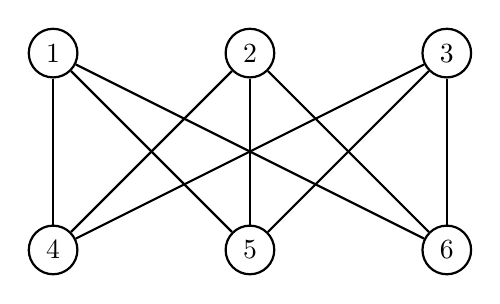
\begin{tikzpicture}[node distance={25mm}, thick, main/.style = {draw, circle}]
              \node[main] (1) {$1$};
              \node[main] (2) [right of=1] {$2$};
              \node[main] (3) [right of=2] {$3$};
              \node[main] (4) [below of=1] {$4$};
              \node[main] (5) [right of=4] {$5$};
              \node[main] (6) [right of=5] {$6$};
              \draw[-] (1) -- (4);
              \draw[-] (1) -- (5);
              \draw[-] (1) -- (6);
              \draw[-] (2) -- (4);
              \draw[-] (2) -- (5);
              \draw[-] (2) -- (6);
              \draw[-] (3) -- (4);
              \draw[-] (3) -- (5);
              \draw[-] (3) -- (6);
          \end{tikzpicture}

          \begin{enumerate}
              \item What is the start state?

                    $M_1: q_1$

                    $M_2: q_1$

              \item What is the set of accept states?
              \item What sequence of states does the machine go through on input $aabb$?
              \item Does the machine accept the string $aabb$?
              \item Does the machine accept the string $\epsilon$?
          \end{enumerate}
\end{enumerate}
